%%%%%%%%%%%%%%%%%%%%%%%%%%%%%%%%%%%%%%%%%%%%%%%%%%%%%%%%%%%%%%%%%%%
%                       DELETED
%%%%%%%%%%%%%%%%%%%%%%%%%%%%%%%%%%%%%%%%%%%%%%%%%%%%%%%%%%%%%%%%%%%

%--------------------------------------------------------------
%       Tabella tempi dei kernel al variare di thread
%           e blocchi del primo macro-modulo
%--------------------------------------------------------------
\subsection{Tempi dei kernel al variare di thread e blocchi per il primo macro-modulo}
\begin{table}[h!]
    \centering
    \begin{tabularx}{1\textwidth} { 
      | >{\centering\arraybackslash}X 
      | >{\centering\arraybackslash}X
      | >{\centering\arraybackslash}X
      | >{\centering\arraybackslash}X
      | >{\centering\arraybackslash}X
      | >{\centering\arraybackslash}X
      | >{\centering\arraybackslash}X|
    }
    \hline Threads & Blocks & \texttt{defineLDiffGPU time (s)} & \texttt{defineLMatrixGPU time (s)} \\
    \hline $10 \times 10$ & $7 \times 7$ & $2.4640 \times 10^{-5}$ & $23.904 \times 10^{-5}$ \\
    \hline $16 \times 16$ & $4 \times 4$ & $2.1760 \times 10^{-5}$ & $11.232 \times 10^{-5}$ \\
    \hline $20 \times 20$ & $4 \times 4$ & $2.4960 \times 10^{-5}$ & $14.048 \times 10^{-5}$ \\
    \hline $32 \times 32$ & $2 \times 2$ & $2.2080 \times 10^{-5}$ & $16.256 \times 10^{-5}$ \\
    \hline
    \end{tabularx}
    \caption{Confronto tempi dei due kernel del primo macro-modulo per $M = 64$} 
    \label{tab:kernels_first_macro_module_time}
\end{table}

% Tabelle
\begin{table}[h!]
    \centering
    \begin{tabularx}{1.0\textwidth} { 
      | >{\centering\arraybackslash}X 
      | >{\centering\arraybackslash}X
      | >{\centering\arraybackslash}X
      | >{\centering\arraybackslash}X
      | >{\centering\arraybackslash}X
      | >{\centering\arraybackslash}X
      | >{\centering\arraybackslash}X
      | >{\centering\arraybackslash}X
      | >{\centering\arraybackslash}X
      | >{\centering\arraybackslash}X|
    }
    \hline
    i & k & j & Y & B & A & Fnm1 & Y & d\\
    \rowcolor{lightgray}
    \hline 1 & 1 & 1 & [1,2] & [1,1] & [1,1] & [1] & [1,1] & 192\\ 
    \hline 1 & 1 & 1 & [1,2] & [1,2] & [1,2] & [193] & [193,1] & 192\\ 
    \rowcolor{lightgray}
    \hline 1 & 1 & 1 & [2,2] & [1,1] & [1,1] & [1] & [1,1] & 192\\ 
    \hline 1 & 1 & 1 & [2,2] & [1,2] & [1,2] & [194] & [194,1] & 192\\ 
    \hline $\vdots$ & $\vdots$ & $\vdots$ & $\vdots$ & $\vdots$ & $\vdots$ & $\vdots$ & $\vdots$ & $\vdots$ \\ 
    \rowcolor{lightgray}
    \hline 1 & 192 & 1 & [192,2] & [1,1] & [1,1] & [192] & [192,1] & 192\\ 
    \hline 1 & 192 & 2 & [192,2] & [1,2] & [1,2] & [384] & [384,1] & 192\\ 
    \hline $\vdots$ & $\vdots$ & $\vdots$ & $\vdots$ & $\vdots$ & $\vdots$ & $\vdots$ & $\vdots$ & $\vdots$ \\
    
    \rowcolor{lightgray}
    \hline 2 & 1 & 1 & [193,2] & [2,1] & [2,1] & [1] & [1,1] & 192\\ 
    \hline 2 & 1 & 1 & [193,2] & [2,2] & [2,2] & [193] & [193,1] & 192\\ 
    \rowcolor{lightgray}
    \hline 2 & 1 & 1 & [194,2] & [2,1] & [2,1] & [2] & [2,1] & 192\\ 
    \hline 2 & 1 & 1 & [194,2] & [2,2] & [2,2] & [194] & [194,1] & 192\\ 
    \hline $\vdots$ & $\vdots$ & $\vdots$ & $\vdots$ & $\vdots$ & $\vdots$ & $\vdots$ & $\vdots$ & $\vdots$ \\ 
    \rowcolor{lightgray}
    \hline 2 & 192 & 1 & [384,2] & [2,1] & [2,1] & [192] & [192,1] & 192\\ 
    \hline 2 & 192 & 2 & [384,2] & [2,2] & [2,2] & [384] & [384,1] & 192\\ 
    \hline
    \end{tabularx}
    \caption{La tabella mostra al variare di $i$, $j$ e $k$ quali sono gli elementi su cui opera la porzione di codice sopra descritta}
    \label{tab:debugging_table}
\end{table}


%>>>>>>>>>>>>>>>>>>>>>>>>>>>>>>>>>>>>>>>>>>>>>>>>>>>>>
%               Delta_t = 1/2^11
%>>>>>>>>>>>>>>>>>>>>>>>>>>>>>>>>>>>>>>>>>>>>>>>>>>>>>
\newpage
\begin{center}
    $\Delta _t = 1 / 2^{11}, N = 102400$    
\end{center}

\begin{table}[h!]
    \centering
    \begin{tabularx}{1\textwidth} { 
      | >{\centering\arraybackslash}X 
      | >{\centering\arraybackslash}X
      | >{\centering\arraybackslash}X
      | >{\centering\arraybackslash}X
      | >{\centering\arraybackslash}X
      | >{\centering\arraybackslash}X
      | >{\centering\arraybackslash}X
      | >{\centering\arraybackslash}X|
    }
    \hline  Threads & Blocks & \texttt{compute One Column GPU chiamate} & \texttt{compute One Column GPU tempo medio (s)} & \texttt{compute Y GPU chiamate} & \texttt{compute Y GPU tempo medio (s)} \\
    \hline $16 \times 1$ & $12 \times 1$ & $513026$ & $2.1700 \times 10^{-5}$ & $409596$ & $3.7320 \times 10^{-5}$ \\
    \hline $20 \times 1$ & $10 \times 1$ & $513026$ & $2.3290 \times 10^{-5}$ & $409596$ & $4.2380 \times 10^{-5}$ \\
    \hline $32 \times 1$ & $6 \times 1$ & $513026$ & $2.7020 \times 10^{-5}$ & $409596$ & $5.6600 \times 10^{-5}$ \\
    \hline $40 \times 1$ & $5 \times 1$ & $512004$ & $2.7520 \times 10^{-5}$ & $409596$ & $5.6950 \times 10^{-5}$ \\
    \hline $64 \times 1$ & $3 \times 1$ & $512004$ & $2.7430 \times 10^{-5}$ & $409596$ & $5.7010 \times 10^{-5}$ \\
    \hline
    \end{tabularx}
    \label{tab:second_macro_module_time_N_102400}
\end{table}
\vspace{0.2cm}

%>>>>>>>>>>>>>>>>>>>>>>>>>>>>>>>>>>>>>>>>>>>>>>>>>>>>>
%               Delta_t = 1/2^12
%>>>>>>>>>>>>>>>>>>>>>>>>>>>>>>>>>>>>>>>>>>>>>>>>>>>>>
\newpage 
\noindent
\begin{center}
    $\Delta _t = 1 / 2^{12}, N = 204800$    
\end{center}

\begin{table}[h!]
    \centering
    \begin{tabularx}{1\textwidth} { 
      | >{\centering\arraybackslash}X 
      | >{\centering\arraybackslash}X
      | >{\centering\arraybackslash}X
      | >{\centering\arraybackslash}X
      | >{\centering\arraybackslash}X
      | >{\centering\arraybackslash}X
      | >{\centering\arraybackslash}X
      | >{\centering\arraybackslash}X|
    }
    \hline  Threads & Blocks & \texttt{compute One Column GPU chiamate} & \texttt{compute One Column GPU tempo medio (s)} & \texttt{compute Y GPU chiamate} & \texttt{compute Y GPU tempo medio (s)} \\
    \hline $16 \times 1$ & $12 \times 1$ & $1025026$ & $2.1670 \times 10^{-5}$ & $819196$ & $3.7380 \times 10^{-5}$ \\
    \hline $20 \times 1$ & $10 \times 1$ & $1025026$ & $2.3290 \times 10^{-5}$ & $819196$ & $4.2440 \times 10^{-5}$ \\
    \hline $32 \times 1$ & $6 \times 1$ & $1025026$ & $2.7030 \times 10^{-5}$ & $819196$ & $5.6660 \times 10^{-5}$ \\
    \hline $40 \times 1$ & $5 \times 1$ & $1024004$ & $2.7520 \times 10^{-5}$ & $819196$ & $5.7040 \times 10^{-5}$ \\
    \hline $64 \times 1$ & $3 \times 1$ & $1024004$ & $2.7450 \times 10^{-5}$ & $819196$ & $5.7080 \times 10^{-5}$ \\
    \hline
    \end{tabularx}
    \label{tab:second_macro_module_time_N_204800}
\end{table}
\vspace{0.2cm}

%>>>>>>>>>>>>>>>>>>>>>>>>>>>>>>>>>>>>>>>>>>>>>>>>>>>>>
%               Delta_t = 1/2^13
%>>>>>>>>>>>>>>>>>>>>>>>>>>>>>>>>>>>>>>>>>>>>>>>>>>>>>
\newpage
\noindent
\begin{center}
    $\Delta _t = 1 / 2^{13}, N = 409600$
\end{center}

\begin{table}[h!]
    \centering
    \begin{tabularx}{1\textwidth} { 
      | >{\centering\arraybackslash}X 
      | >{\centering\arraybackslash}X
      | >{\centering\arraybackslash}X
      | >{\centering\arraybackslash}X
      | >{\centering\arraybackslash}X
      | >{\centering\arraybackslash}X
      | >{\centering\arraybackslash}X
      | >{\centering\arraybackslash}X|
    }
    \hline  Threads & Blocks & \texttt{compute One Column GPU chiamate} & \texttt{compute One Column GPU tempo medio (s)} & \texttt{compute Y GPU chiamate} & \texttt{compute Y GPU tempo medio (s)} \\
    \hline $16 \times 1$ & $12 \times 1$ & $2049026$ & $2.1690 \times 10^{-5}$ & $1638396$ & $3.7420 \times 10^{-5}$ \\
    \hline $20 \times 1$ & $10 \times 1$ & $2049026$ & $2.3290 \times 10^{-5}$ & $1638396$ & $4.2420 \times 10^{-5}$ \\
    \hline $32 \times 1$ & $6 \times 1$ & $2049026$ & $2.7030 \times 10^{-5}$ & $1638396$ & $5.6690 \times 10^{-5}$ \\
    \hline $40 \times 1$ & $5 \times 1$ & $2048004$ & $2.7520 \times 10^{-5}$ & $1638396$ & $5.7040 \times 10^{-5}$ \\
    \hline $64 \times 1$ & $3 \times 1$ & $2048004$ & $2.7450 \times 10^{-5}$ & $1638396$ & $5.7080 \times 10^{-5}$ \\
    \hline
    \end{tabularx}
    \label{tab:second_macro_module_time_N_409600}
\end{table}
\vspace{0.2cm}

%>>>>>>>>>>>>>>>>>>>>>>>>>>>>>>>>>>>>>>>>>>>>>>>>>>>>>
%               Delta_t = 1/2^14
%>>>>>>>>>>>>>>>>>>>>>>>>>>>>>>>>>>>>>>>>>>>>>>>>>>>>>
\newpage
\noindent
\begin{center}
    $\Delta _t = 1 / 2^{14}, N = 819200$ 
\end{center}

\begin{table}[h!]
    \centering
    \begin{tabularx}{1\textwidth} { 
      | >{\centering\arraybackslash}X 
      | >{\centering\arraybackslash}X
      | >{\centering\arraybackslash}X
      | >{\centering\arraybackslash}X
      | >{\centering\arraybackslash}X
      | >{\centering\arraybackslash}X
      | >{\centering\arraybackslash}X
      | >{\centering\arraybackslash}X|
    }
    \hline  Threads & Blocks & \texttt{compute One Column GPU chiamate} & \texttt{compute One Column GPU tempo medio (s)} & \texttt{compute Y GPU chiamate} & \texttt{compute Y GPU tempo medio (s)} \\
    \hline $16 \times 1$ & $12 \times 1$ & $4097026$ & $2.1680 \times 10^{-5}$ & $3276796$ & $3.7400 \times 10^{-5}$ \\
    \hline $20 \times 1$ & $10 \times 1$ & $4097026$ & $2.3290 \times 10^{-5}$ & $3276796$ & $4.2440 \times 10^{-5}$ \\
    \hline $32 \times 1$ & $6 \times 1$ & $4097026$ & $2.7020 \times 10^{-5}$ & $3276796$ & $5.6680 \times 10^{-5}$ \\
    \hline $40 \times 1$ & $5 \times 1$ & $4096004$ & $2.7510 \times 10^{-5}$ & $3276796$ & $5.7040 \times 10^{-5}$ \\
    \hline $64 \times 1$ & $3 \times 1$ & $4096004$ & $2.7460 \times 10^{-5}$ & $3276796$ & $5.7100 \times 10^{-5}$ \\
    \hline
    \end{tabularx}
    \label{tab:second_macro_module_time_N_819200}
\end{table}
\vspace{0.2cm}

%--------------------------------------------------------------
%                   computeOneColumnGPU
%--------------------------------------------------------------
\subsubsection{computeOneColumnGPU}
\noindent La necessità di questo kernel nasce dal fatto che la maggior parte delle operazioni svolte in questo macro-modulo coinvolgono una colonna di varie matrici di appoggio. Sfruttando quindi il parallelismo dell'architettura CUDA, si vuole fare in modo di distribuire il compito di inizializzare una colonna tra vari thread e blocchi. Poiché si è preferito allocare tutte le matrici per righe e dunque considerarle come array, per muoversi lungo le colonne risulta indispensabile il valore denominato leading dimension, abbreviato in ld. Nel caso del C/C++, dove le matrici sono allocate per righe in memoria, la leading dimension è rappresentata dal numero di colonne della matrice. In altri linguaggi di programmazione, come ad esempio il Fortran, le matrici sono allocate per colonne e dunque la leading dimension è rappresentata dal numero di righe. Fissato un numero di thread, verrà ricavato un opportuno numero di blocchi e ciascun thread provvederà all'inizializzazione della colonna come schematizzato nella Figura \ref{fig: computeOneColumnGPU-data-distribution}.

\begin{figure}[h!]
    \centering
    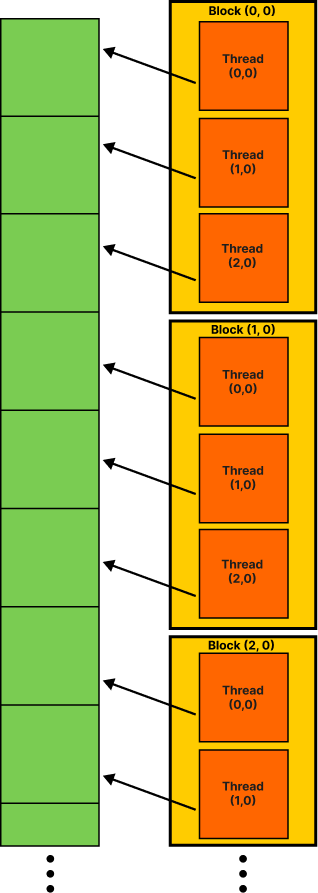
\includegraphics[scale=0.3]{img/computeOneColumnGPU.png}
    \caption{Distribuzione del lavoro tra i thread per il kernel computeOneColumnGPU}
    \label{fig: computeOneColumnGPU-data-distribution}
\end{figure}

\noindent Per rendere il kernel quanto più generale possibile, i parametri di input sono:
\begin{itemize}
    \item matrice A, la matrice di output
    \item dimensioni matrice A
    \item leading dimension di A
    \item matrice B, la matrice di input
    \item leading dimension di B
\end{itemize}

\noindent Dato che anche le matrici sono allocate come vettori, $A$ e $B$ possono essere o matrici o vettori con l'unica accortezza che quando si passa un vettore al kernel, bisogna impostare la leading dimension a 1.

%--------------------------------------------------------------
%                   computeYGPU
%--------------------------------------------------------------
\subsubsection{computeYGPU}
\noindent Questo kernel ha il compito di parallelizzare il calcolo di $Y$ che rappresenta la soluzione finale del problema. La strategia di parallelizzazione è stata creata analizzando la seguente porzione di codice:

\begin{lstlisting}[language=Matlab]
for i = 1:s
    for k = 1:d
        for j = 1:s
            Y((i-1)*d+k,n) = Y((i-1)*d+k,n) + B(i,j)*Y((j-1)*d+k,n-1) + h*A(i,j)*Fnm1((j-1)*d+k);
        end
    end
end
\end{lstlisting}

\noindent Per prima cosa, è stata realizzata la Tabella, che mostra al variare di $i$, $j$ e $k$ quali sono gli elementi di $Y$, $A$, $B$ e $Fnm1$ a cui la porzione di codice accede. Dunque i parametri di input saranno $Y$, $Fnm1$, $A$ e $B$ con le relative dimensioni e leading dimension per ogni struttura dati.\\ 
Il kernel, di per sé, consiste semplicemente nell'eseguire l'operazione che si trova nel ciclo for più interno su una colonna della matrice $Y$, ma richiamandolo due volte con i parametri di input opportunamente configurati, si eseguiranno prima le operazioni che si trovano sulle righe di colore grigio e poi quelle che si trovano sulle righe di colore bianco. \\
Infatti, possiamo osservare ad esempio che quando $i = 1$ si opera sui primi 191 elementi della $n-1$-esima colonna di $Y$ e i primi 191 elementi del vettore $Fnm1$, ma quando $i = 2$ (e quindi a $s$), si operano sui restanti 191 elementi delle due strutture dati. Sempre quando $i = 1$ si opera sugli elementi $B[0, 0]$ e $A[1, 0]$ delle due matrici e quando $i = 2$ si opera su $B[0, 1]$ e $A[1, 1]$. Difatti, operando in questo modo, si vanno a parallelizzare i due cicli for più interni, cioè quelli in $k$ e in $j$ mentre il ciclo for più esterno deve essere per forza eseguito in sequenziale. \\
Nella sezione successiva verranno analizzati con grande dettaglio i tempi ottenuti dai due kernel del secondo macro-modulo stavolta non solo al variare delle diverse configurazioni di thread e blocchi, ma anche al variare di $\Delta _t$ e conseguentemente $N$.